\section{Multi-core architecture and evolution}



\subsection{SMP}
\label{sec:smp}


%   (-_-)   %
\begin{figure}[!ht]
        \centering
        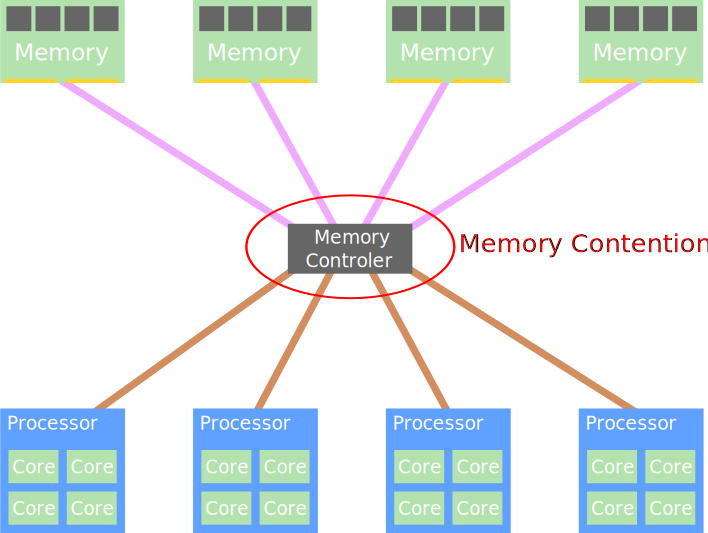
\includegraphics[width=0.8\textwidth]{smp}
        \caption{Overview of an Uniform Memory Access architecture}
        \label{fig:smp}
\end{figure}



\subsection{NUMA}
%   (-_-)   %
\begin{figure}[!ht]
  \centering
  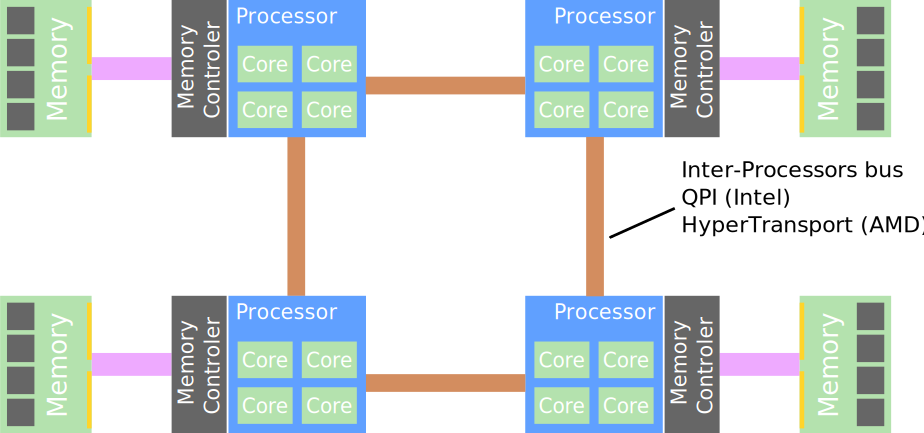
\includegraphics[width=\textwidth]{numa}
  \caption{Overview of an NUMA architecture}
  \label{fig:numa}
\end{figure}



\subsection{Many-core architecture}


Another solution, used by Intel in Xeon Phi coprocessor, is to use a ring bus (See Fig~\ref{fig:interconnect}).
%
Memory is distributed over the ring bus just as core units.
%

%   (-_-)   %
\begin{figure}[!ht]
  \centering
  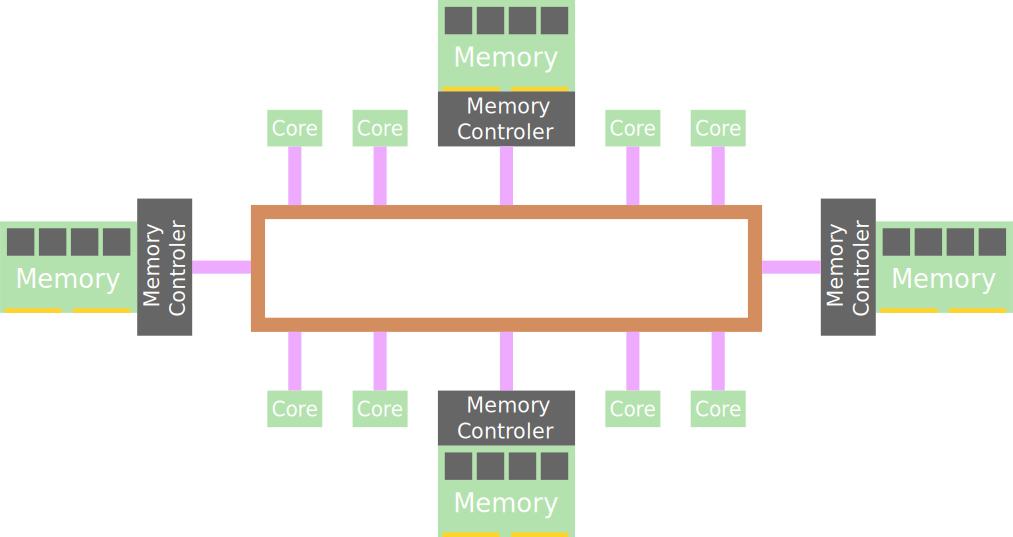
\includegraphics[width=\textwidth]{interconnect}
  \caption{Overview of Xeon Phi Architecture}
  \label{fig:interconnect}
\end{figure}
